\section{Calculus}\label{sec:calculus}

In this section, we define a calculus that formally describes the operational semantics
of speculative nondeterminism. We first present the data models of the framework which
is independent of the rest of the calculus. Then we introduce the syntax of the language,
its typing and evaluation rules, and finally we discuss the exit and commit semantics
which are most interesting aspects of the framework.

\subsection{Data Model}\label{sec:datamodel}

Speculative nondeterminism is a programming framework that assumes a centralized
data store that acts as the primary programming environment. The implementation of this store is
not part of the language and therefore independent from the operational semantics of the language.
Here we present the abstract data model of the store that can be instantiated into different
concrete models.
%Typical examples of a data model are tuple space, record space, key-value store, relational model (relations), and logic programs (predicates).
%New data models can also be customized for domain-specific applications and be built on top of existing data models.
%The data model is separated from the speculative choices, which means the data
%model can be changed without affecting the behavior of speculations as long
%as the data model provides the features needed by speculation.

A data model is a 8-tuple
$$\dm=\langle\mkstore,\alltype,\allop,\allstore,\dstype,\vdash,\sqcup,\dtrans\rangle$$
where
\begin{description}
  \item[$\mkstore$] defines an empty data store.
  \item[$\alltype$] is the set of all types available in the data model.
  \item[$\allop$] is the set of all data operations available in the data model.
  \item[$\allstore$] is the set of all possible data stores.
  \item[$\dptype:\allop\to\alltype$] returns the type of an operation.
  \item[$\dstype:\allstore\to 2^\alltype$] returns the set of types of a data store; $\dstype(\mkstore)=\emptyset$.
  \item[$\vdash\subseteq\allstore\times\allop$] is a binary relation
denoted by $d\vdash p$.
It defines when operation $p$ can be executed on the data store $d$.
For example, if the operation $p$ has a precondition, $d\vdash p$ is
true if and only if the condition is true when evaluated on the data store $d$.
  \item[$\sqcup:\allstore\times\allstore\to\allstore$] is a disjoint union function
such that for $d_1\sqcup d_2$, $\dstype(d_1)\cap\dstype(d_2)=\emptyset$.
The disjoint requirement is needed to guarantee safe merge of two stores.
As an example, two key-value stores with overlapped types,
$[a\mapsto 1]$ and $[a\mapsto 2]$, cannot be merged together.
  \item[$\dtrans:\allop\times\allstore\to\allstore$] is the transition function that
defines the effect of data operations on the store. 
It should be guaranteed that $\dstype(\dtrans(p,d))\subseteq\{\dptype(p)\}\cup\dstype(d)$. 
\end{description}

Next we give some examples of concrete data models under the above framework.

\subsubsection*{Data Model for Dining Philosophers Problem}

It's easier to represent the 3 Dining Philosophers Problem with
a customized data model defined below.
A data store is essentially a set of forks on the table. 
This data model assumes just one dining table for brevity.
\begin{align*}
  \mkstore &= \emptyset
\\
  \alltype &= \{ x,y,z \}
\\
  \allop &= \{ -x, -y, -z, +x, +y, +z \}
\\
  \allstore &= 2^\alltype
\\
  \dptype(-w) & =\dptype(+w)=w \text{ where } w\in\alltype
\\
  \dstype(d) &= \alltype
\\
  % \frac{w\in d}{d\vdash -w}, &
  % \hspace*{1ex} \frac{}{d\vdash +w}
  % \text{ where } w\in\alltype
  \vdash &= \{(d,-w):w\in d\}\cup\{(d,+w):w\in\alltype\}
\\
%  d_1\sqcup d_2 & = d_1\cap d_2
%  \\&\text{\em $\sqcup$ merges two data stores by taking the intersection of}
%  \\&\text{\em the two sets, because for example $A$ grabs $x$ and $d_1=$}
%  \\&\text{\em $\{y,z\}$, and $B$ in another galaxy has $d_2=\{x,y,z\}$ and}
%  \\&\text{\em wants to merge with $d_1$, only intersection can correctly}
%  \\&\text{\em merge them.}
  d_1\sqcup d_2 & = d_1\cup d_2
\\
  \dtrans(-w,d) &= d\setminus\{w\},
  \dtrans(+w,d) = d\cup\{w\}
  \text{ where } w\in\alltype
\end{align*}
It is possible to execute $-w$ (to grab the fork $w$) only if $w\in d$ (the fork $w$ is on the table).
To grab a fork $w$ ($-w$) is to remove $w$ from the set $d$, and to put down a fork $w$ ($+w$) is to add $w$ to the set $d$.

\subsubsection*{Tuple Space}

The idea of tuple space comes from Linda \cite{Gelernter85:Linda}, where
a tuple space is a multi-set of tuples that can be accessed concurrently.
Agents can post their data to the tuple space in the form of tuples, and retrieve tuples as data from the tuple space that match a certain pattern.
There are three major operations in the tuple space data model:
\begin{description}
\item[$in$] reads and removes a tuple from a tuple space
\item[$out$] produces a tuple, writing it into a tuple space
\item[$rd$] non-destructively reads a tuple space and gets a copy of a tuple
\end{description}
Formal definitions and operational semantics for
the $in/out/rd$ operations are provided in \cite{Ciancarini95}
which can be easily adapted to this framework.

%\begin{example}[Tuple Space for Trading]
%Data models can not only be customized for domain-specific purposes, as shown in Section \ref{sec:custom3dp},
%but also be built on top of existing data models.
%In this example, two primitive operations for trading, $buy$ and $sell$, are implemented on top of the tuple space data model.
%Only the availability and the type of products being traded are considered, while the prices are ignored for simplicity.
%\setcounter{equation}{0}
%\begin{eqnarray}
%sell(t:\textbf{Product}) :=
%& \mathbf{let} & id=new\_trans\_id() \label{eg:trade:sell:1}\\
%& \mathbf{in}  & out(t,\textbf{sell},id) \label{eg:trade:sell:2} \\
%&     & in(t,\textbf{buy},id) \label{eg:trade:sell:3} \\
%&     & out(t,\textbf{ack},id) \label{eg:trade:sell:4} \\
%buy(t:\textbf{Product}) :=
%& \mathbf{let} & id:\mathbf{integer} \label{eg:trade:buy:1} \\
%& \mathbf{in}  & in(t,\textbf{sell},\mathbf{ref}~id) \label{eg:trade:buy:2} \\
%&     & out(t,\textbf{buy},id) \label{eg:trade:buy:3} \\
%&     & rd(t,\textbf{ack},id) \label{eg:trade:buy:4}
%\end{eqnarray}
%
%As shown above, both $sell$ and $buy$ are presented in pseudo-code form and make use of primitive operations in the tuple space data model such as $in$, $out$ and $rd$.
%
%First we explain the $sell$ operation.
%The function $new\_trans\_id$ allocates a unique transaction number in the form of an integer (line \ref{eg:trade:sell:1}).
%Then a tuple of the product type $t$, the trade type $\textbf{sell}$ and the transaction number $id$ is posted to the tuple space (line \ref{eg:trade:sell:2}).
%Later it waits for a tuple of trade type $\textbf{buy}$ to appear and consumes it by using the $in$ operation (line \ref{eg:trade:sell:3}).
%Finally, it produces an acknowledgement of the transaction being completed (line \ref{eg:trade:sell:4}).
%
%The $buy$ operation is similar to $sell$.
%First the variable $id$ is declared to be an integer (line \ref{eg:trade:buy:1}).
%Next it waits for a tuple of trade type $\textbf{sell}$, which is produced elsewhere in line \ref{eg:trade:sell:2}, and consumes it, filling $id$ with the value of the third element in the tuple (line \ref{eg:trade:buy:2}).
%Then it produces a tuple of trade type $\textbf{buy}$ (line \ref{eg:trade:buy:3}), which will be consumed later in line \ref{eg:trade:sell:3}.
%Finally the acknowledgement is read for confirmation of the completion (line \ref{eg:trade:buy:4}).
%\end{example}

\subsubsection*{Key-value Store}

{\em Key-value store} is a mapping from arbitrary names
(i.e. keys) to arbitrary values.
For example, $[a\mapsto 3, b\mapsto 5]$ is a key-value store
where the key $a$ gets value $3$ and $b$ gets $5$.
The set of types of a key-value store is the set of names in
the store ($\{a,b\}$ in the example). The scope of data operations normally
includes (i) creating a new key-value pair,
(ii) updating an existing key with a new value,
(iii) getting a value according to a key, and
(iv) removing a key and its corresponding value.
Conditional guards can also be combined with these data operations,
e.g., $a>4\Rightarrow b\gets 2$ waits (blocks) until
the condition $a>4$ is true in the store,
and then updates the value of $b$ to $2$.

\subsubsection*{Other Models}
Other more structured data models include relational data and logic programs.
Data operations are insertion and deletion of tuples/predicates. Applications
using these models are also typical.

%{\em Relational model} is a classic and powerful data model. Data is represented by tuples and grouped into relations according to their domain-specific meanings.
%    Conventionally, relations and tuples can be manipulated by using relational algebra or SQL,
%    which is also viable in our framework being the data operation.
%    The types in this relational data model are the relation names,
%    or relation names together with specific ranges of values on a field in condition of data fragmentation.
%
%{\em Logical predicates} can also be used as a data model which can support a knowledge base for inferences.
%The scope of data operations in a logical predicates data model includes monotonically adding rules/facts to the knowledge base, and asking for an evaluation of a predicate.
%


\subsection{Syntax, Typing and Basic Operations}\label{sec:rules}

\begin{figure}
  \centering
  \begin{eqnarray*}
    a & ::= & [e,f] \text{ where } f:\allstore\to\nat \\
    e & ::= & e_1 \oplus e_2 \\ 
      &   | & e_1 . e_2 \\
      &   | & p \text{ where } p\in\allop \\
      &   | & \cm  ~~|~~ \cu  ~~|~~ \epsilon \\
      &     & \\
    U & ::= & \emptyset \\
      &   | & \{G_1,\dots,G_n\} \\
    G & ::= & \langle A,d,s \rangle \text{ where } d\in\allstore, s\in2^{\nat\times\nat} \\
      &   | & G_1 \oplus_k G_2 \text{ where $k\in\nat$ is the identifier of an agent} \\
    A & ::= & [] \\
      &   | & [a_1,\dots,a_m]
  \end{eqnarray*}
  \caption{Syntax and Runtime Data Structures}
  \label{fig:syntax}
\end{figure}

\figref{fig:syntax} first gives the syntax of agent programs 
for a data model.
\begin{description}
\item[$a$] is an agent $[e,f]$ where $e$ is the program and
	$f$ is the exit condition function.
\item[$e_1\oplus e_2$] is the exclusive choice construct.
\item[$e_1.e_2$] is the execution of $e_1$ and $e_2$ in a sequence.
\item[$p\in\allop$] is the data operation defined in the data model.
\item[$\epsilon$] is an empty program indicating the end of a program.
\item[$\cm$ and $\cu$] are primitives for pruning choices, which are described briefly in Section \ref{sec:overview} and formally in Section \ref{sec:commit2}. A well-formed program must have a matching $\cm$ for each choice construct.
However, our semantics framework can both add missing $\cm$'s and ignore redundant $\cm$'s automatically.
\end{description}

\figref{fig:syntax} also defines the runtime data structures 
in the calculus.
\begin{description}
\item[$U$] is a universe, the the top-level structure consisting of a set of galaxies.
The initial state of the universe is $\emptyset$.
\item[$G$] is the galaxy which is either a tree of worlds, or just one world.
A world is a quadruple $\langle A, d, s\rangle$ where $A$
is the list of agents participating in this world,
$d$ is the associated data store,
%$c$ is the set of indices (i.e., numeric identifiers) of committed agents,
and $s$ is the map from agent index to the exit value.
\end{description}

For simplicity we use numeric identifiers for agents throughout this paper.
We also use the following notations for the operations of a list:
(i) $|A|$ is the \emph{length} of the list $A$;
(ii) $A[\cdot]$ means \emph{indexing};
(iii) $A[i\mapsto a]$ replaces the $i$-th element of $A$ with $a$;
(iv) $A+B$ is the \emph{concatenation} of list $A$ and list $B$.

Top of \figref{fig:rules} shows the typing rules of the universe and galaxies.
$\typeof\cdot$ is a set of types which are defined in the given data model.
The set of types of the universe is the union of the sets of types of all the galaxies, 
while the set of types of a galaxy is the union of the sets of types of all the leaf worlds. 
Note that all the types come from the data model.

\begin{figure*}
\begin{minipage}{\textwidth}
  \flushright\fbox{$T=S$} \\
  \begin{minipage}{0.24\textwidth}
    \begin{gather*}
    \frac{}{\typeof U = \bigcup_{G\in U} \typeof G} \\
    \frac{
        {a=[e,f]}\qquad
        {\typeof e = \tau_1}}
      {\typeof a = \tau_1}
    \end{gather*}
  \end{minipage}
  \begin{minipage}{0.24\textwidth}
    \begin{gather*}
    \frac{
        {G = \langle A,d,s\rangle}\quad
        {\dstype(d) = \tau_1}}
    {\typeof{G} = \tau_1} \\
    \frac{
        {\typeof{e_1} = \tau_1}\qquad
        {\typeof{e_2} = \tau_2}}
    {\typeof{e_1\oplus e_2} = \tau_1\cup\tau_2}
    \end{gather*}
  \end{minipage}
  \begin{minipage}{0.24\textwidth}
    \begin{gather*}
    \frac{
        {\typeof{G_1} = \tau_1}\qquad
        {\typeof{G_2} = \tau_2}}
    {\typeof{G_1\oplus G_2} = \tau_1\cup\tau_2} \\
    \frac{
        {\typeof{e_1} = \tau_1}\qquad
        {\typeof{e_2} = \tau_2}}
    {\typeof{e_1.e_2} = \tau_1\cup\tau_2}
    \end{gather*}
  \end{minipage}
  \begin{minipage}{0.12\textwidth}
    \begin{gather*}
    \frac{p \in \allop}{\typeof{p} = \{\dptype(p)\}} \\
    \frac{\quad}{\typeof{\cm} = \emptyset}
    \end{gather*}
  \end{minipage}
  \begin{minipage}{0.12\textwidth}
    \begin{gather*}
    \frac{\quad}{\typeof{\epsilon} = \emptyset} \\
    \frac{\quad}{\typeof{\cu} = \emptyset}
    \end{gather*}
  \end{minipage}
  %%%%
  \flushright\fbox{$U+a\Longrightarrow U'$}
  \[
    \tag{\sc Entrance}\label{rule:birth}
    \frac{}{U + a \Longrightarrow U\cup\{\langle [a],\mkstore,\emptyset,\emptyset\rangle\}}
  \]
  \flushright\fbox{$U\uto U'$}
  \[
    \tag{\sc Merge}\label{rule:merge}
    \frac{
    {\begin{matrix}
              w=\langle A,d,s\rangle \\
              w'=\langle A[i\mapsto[e,f]],d',s'\rangle \\
              s'=\snapshot(s,|e|,i,f(d'))
            \end{matrix}}
            \qquad
    {\begin{matrix}
              G,G'\in U \\
              w\in leaves(G)
            \end{matrix}}
            \qquad
    {\begin{matrix}
              p\in\allop \\
              d\vdash p \\
              d'=\dtrans(p,d)
            \end{matrix}}
            \qquad
    {\begin{matrix}
              {\begin{matrix}
                [p.e,f] = A[i] \\
                \dptype(p)\in\typeof{G'}
              \end{matrix}}
              \qquad
              (1\le i\le |A|)
            \end{matrix}}}
    {U \uto (U\setminus\{G,G'\}) \cup \{\gmerge(replace(G,w,w'),G')\}}
  \]
  \[
    \tag{\sc Alone}\label{rule:alone}
    \frac{
    {\begin{matrix}
              w=\langle A,d,s\rangle \\
              w'=\langle A[i\mapsto[e,f]],d',s'\rangle \\
              s'=\snapshot(s,|e|,i,f(d'))
            \end{matrix}}
            \qquad
    {\begin{matrix}
              G\in U \\
              w\in leaves(G)
            \end{matrix}}
            \qquad
    {\begin{matrix}
              p\in\allop \\
              d\vdash p \\
              d'=\dtrans(p,d)
            \end{matrix}}
            \qquad
    {\begin{matrix}
              {\begin{matrix}
                [p.e,f] = A[i] \\
                \dptype(p)\not\in\typeof{U\setminus\{G\}}
              \end{matrix}}
              \qquad
              (1\le i\le |A|)
            \end{matrix}}}
    {U \uto (U\setminus\{G\}) \cup \{replace(G,w,w')\}}
  \]
%
  \flushright\fbox{$G\gto G'$}\\
  \begin{minipage}{0.59\textwidth}
  \[
    \tag{\sc Fork}\label{rule:fork}
    \frac{
    {[(e_1\oplus e_2).e,f]=A[i]}\qquad
%    {H=A[1..i-1]+A[i+1..|A|]}\quad
%    {c'=shiftc(c,i)}\quad
%    {s'=rs(s,i,|A|)}\quad
    {(1\le i\le |A|)}}
    {\langle A,d,s\rangle \gto
      \langle A[i\mapsto[e_1.e,f]],d,s\rangle \oplus_i
      \langle A[i\mapsto[e_2.e,f]],d,s\rangle}
  \]
  \[
    \tag{\sc Cm}\label{rule:cm}
    \frac{
    {[\cm.e,f]=A[i]}\qquad
%    {\{i+1,\dots,|A|\}\subseteq c}\qquad
    {(1\le i\le |A|)}}
    {G\oplus_i\langle A,d,s\rangle \gto \langle A[i\mapsto[e,f]],d,\snapshot(s,|e|,i,f(d))\rangle}
  \]
  \end{minipage}
  \begin{minipage}{0.4\textwidth}
  \[
    \tag{\sc Swap}\label{rule:swap}
    \frac{}{G_1\oplus_k G_2 \gto G_2\oplus_k G_1}
  \]
  \[
    \tag{\sc Cu}\label{rule:cu}
    \frac{
    {[\cu.e,f]=A[i]}\qquad
    {(1\le i\le |A|)}}
    {\langle A,d,s\rangle\oplus_k G \gto G}
  \]
  \end{minipage}
  \vspace{1ex}
  \[
    \tag{\sc Cm-Auto}\label{rule:cm-auto}
    \frac{
      w\in leaves(G) \qquad
      w=\langle A,d,s\rangle \qquad
      [\epsilon,f]=A[i] \qquad
      i\in cid(G) \qquad
      w'=\langle A[i\mapsto[\cm,f]],d,s\rangle \qquad
      (1\le i\le |A|)
    }
    {G \gto replace(G,w,w')}
  \]
  \[
    \tag{\sc Cm-Skip}\label{rule:cm-skip}
    \frac{
      w\in leaves(G) \qquad
      w=\langle A,d,s\rangle \qquad
      [\cm.e,f]=A[i] \qquad
      i\not\in cid(G) \qquad
      w'=\langle A[i\mapsto[e,f]],d,s\rangle \qquad
      (1\le i\le |A|)
    }
    {G \gto replace(G,w,w')}
  \]
  \vspace{1ex}
  \[
    \tag{\sc Exit}\label{rule:exit}
    \frac{%\displaystyle
    W=leaves(G)
    \qquad \sum_{w\in W} ins(w,i)=0
    \qquad i\not\in cid(G)
    \qquad \left|\bigcup_{w\in W} \{exitval(w,i)\}\right|=1
    \qquad (1\le i\le\max_{w\in W} |w|)}
    {G \gto remove(G,i)}
  \]
  \vspace{1mm}
\end{minipage}
%
\begin{minipage}{0.49\textwidth}\centering
  \begin{gather*}
%    \frac{c'=\{j\in c:j<i\}\cup\{j-1:j\in c \land j>i\}}{shiftc(c,i) = c'} \\
    \frac{s'=\{\langle j,v\rangle\in s:j<i\}\cup\{\langle j-1,v\rangle:\langle j,v\rangle\in s \land j>i\}}{shifts(s,i) = s'}
%    \frac{i\in c}{rc(c,i,m) = shiftc(c,i) \cup \{m\}} \qquad
%    \frac{i\not\in c}{rc(c,i,m) = shiftc(c,i)} \\
%    \frac{\langle i,v\rangle\in s}{rs(s,i,m) = shifts(s,i) \cup \{\langle m,v\rangle\}} ~
%    \frac{i\not\in\{j:\langle j,v\rangle\in s\}}{rs(s,i,m) = shifts(s,i)}
  \end{gather*}
  \begin{gather*}
    \frac{\langle G',r\rangle = rg(G,w,w')}
    {replace(G,w,w') = G'} \\
    \frac{\langle G_1',\textbf{true}\rangle = rg(G_1,w,w')}
    {rg(G_1\oplus_k G_2,w,w') = \langle G_1'\oplus_k G_2,\textbf{true}\rangle} \\
    \frac{\langle G_1',\textbf{false}\rangle = rg(G_1,w,w') \qquad \langle G_2',r\rangle = rg(G_2,w,w')}
    {rg(G_1\oplus_k G_2,w,w') = \langle G_1'\oplus_k G_2',r\rangle} \\
    \frac{}{rg(w,w,w') = \langle w',\textbf{true}\rangle} \qquad
    \frac{w_1\ne w}{rg(w_1,w,w') = \langle w_1,\textbf{false}\rangle}
  \end{gather*}
  \[
  % exitval
    %\tag{\sc EVal}
    \frac{w=\langle A,d,s\rangle \qquad \langle i,v\rangle\in s}
    {exitval(w,i)=v}
  \qquad
    \frac{w=\langle A,d,s\rangle}{|w|=|A|}
  \]
  \[
    \frac{}{\snapshot(s,0,i,v)=s\cup\{\langle i,v\rangle\}}
    \qquad
    \frac{l>0}{\snapshot(s,l,i,v)=s}
  \]
  \begin{gather*}
    \frac{}{|e_1\oplus e_2|=\max(|e_1|,|e_2|)}
    \qquad
    \frac{}{|e_1.e_2|=|e_1|+|e_2|}
  \\
    \frac{p\in\allop}{|p|=1}
    \qquad
    \frac{}{|\epsilon|=0}
    \qquad
    \frac{}{|\cm|=1}
    \qquad
    \frac{}{|\cu|=1}
  \end{gather*}
\end{minipage}
\hspace{5mm}
\begin{minipage}{0.49\textwidth}\centering
  %% galaxy merging functions
  \begin{gather*}
    \frac
      {G=G_1\oplus_k G_2}
      {\gmerge(G,G')=\gmerge(G_1,G')\oplus_k\gmerge(G_2,G')}
  \\
    \frac{}{\gmerge(w,G')=\gpaste(w,G')}
  \end{gather*}
  \begin{gather*}
    \frac
      {w=\langle A,d,s\rangle
      \qquad
      G=G_1\oplus_k G_2}
      {\gpaste(w,G)=\gpaste(w,G_1)\oplus_{k+|w|}\gpaste(w,G_2)}
  \\
    \frac
      {\begin{matrix}
        w=\langle A_0,d_0,s_0\rangle \qquad
        G=\langle A,d,s\rangle \\
        s'=s_0\cup\{\langle i+|w|,v\rangle:\langle i,v\rangle\in s\}
      \end{matrix}}
      {\gpaste(w,G)=\langle A_0+A,d_0\sqcup d,s'\rangle}
  \end{gather*}
  %%
  \[
    \frac{}{cid(G_1\oplus_k G_2)=cid(G_1)\cup cid(G_2)\cup\{k\}} \qquad
    \frac{}{cid(w)=\emptyset}
  \]
  %% Auxiliary Functions for Exit Inference Rules
  \[
  % leaves
    \frac{G=G_1\oplus_k G_2}{leaves(G)=leaves(G_1)\uplus leaves(G_2)}
    \quad
    \frac{}{leaves(w)=\lbb w\rbb}
  \]
  \[
  % #instr
    \frac{w=\langle A,d,s\rangle \qquad [e,f]=A[i] \qquad (1\le i\le |A|)}
    {ins(w,i)=|e|}
  \]
  \begin{gather*}
  % remove
    \frac{G=G_1\oplus_k G_2}
    {remove(G,i)=remove(G_1,i)\oplus_k remove(G_2,i)}
  \\
    \frac{\begin{matrix}
        w=\langle A,d,s\rangle \qquad
%        c'=shiftc(c,i) \qquad
        s'=shifts(s,i)
    \end{matrix}}
    {remove(w,i)=\langle A[1..i-1]+A[i+1..|A|],d,s'\rangle}
  \end{gather*}
\end{minipage}
%
  \caption{Inference Rules}
  \label{fig:rules}
\end{figure*}

\figref{fig:rules} shows all the inference rules used to implement our framework.
The system starts with an empty universe $\emptyset$.
New agents can dynamically enter the system via the $+$ operator.
The entrance of a new agent will create a galaxy with one world by itself,
as shown in \ref{rule:birth}.

When one of the agents is ready to execute some operation $p$
on the data store $d$ (i.e., $d\vdash p$),
rules \ref{rule:merge} and \ref{rule:alone} force the checking of
types involved in that operation.
As mentioned in Section \ref{sec:overview},
worlds are partitioned into galaxies according
to the interests of their associated agents at run-time.
The interest is, in fact, the types here.
\ref{rule:merge} shows the case when the type of the operation $p$
interleaves with the type of galaxy $G'$.
In this case, the current galaxy $G$, has to be merged with the galaxy $G'$,
which contains the required type.
In case there is no need to merge with other galaxies,
i.e., either the type resides in the current galaxy or it is a new type,
the operation $p$ is executed directly,
as shown in rule \ref{rule:alone}.

The main idea of speculative nondeterminism is forking and pruning of choices.
\ref{rule:fork} fires if an agent is reduced to
a choice $(e_1\oplus e_2) .e$,
and it consumes the choice construct in the agent to split the current world of
the agent into two.
When the agent on the lowest level of the galaxy tree structure
executes $\cm$, as shown in rule \ref{rule:cm},
the other side of the choice is pruned.
Similarly, for $\cu$ operations, the current side of the choice is pruned instead,
as shown in rule \ref{rule:cu}.
The key difference between $\cm$ and $\cu$ is that
$\cu$ can be executed in any agent and cause the pruning to takes place immediately,
while $\cm$ can only be executed in the lowest-level agents which are
more localized and less aggressive.
Also $\cm$ is blocking when it is not on the lowest level of the tree,
because non-blocking $\cm$ here potentially consumes more resources 
under the risk of being pruned by the $\cm$ on the lowest level. 
This form of commit semantics is therefore known as \emph{localized commit},
which is described in more details in Section \ref{sec:commit2}.
Finally, the rule \ref{rule:cm-auto} automatically adds a $\cm$ at the end of a program 
in case the program is ill-formed and doesn't have a commit operator that matches
a choice. 
Rule \ref{rule:cm-skip} handles another kind of ill-formed program where
there is more than one $\cm$ for a choice branch. 
In this case, only the first $\cm$ is honored but all subsequent ones are ignored.
We don't need a similar skip rule for $\cu$ because the first $\cu$ in a branch
already prunes the current branch.

Rules without names define the following auxiliary functions.
\begin{description}
\item[$shifts(s,i)$] removes the snapshot of $i$ (i.e. $\langle i,v\rangle$) from $s$ (if applicable) and shifts the indices by 1 of snapshots with index greater than $i$.
A \emph{snapshot} is a pair $\langle i,v\rangle$ where $i$ is an agent's index, and $v$ is the evaluation result of the exit condition function $f_i$ of the agent $i$ at the point of time when agent $i$ finishes execution.
\item[$replace(G,w,w')$] replaces world $w$ in galaxy $G$ with $w'$.
\item[$rg(G,w,w')$] is a helper function for $replace$.
\item[$\gmerge(G,G')$] merges 2 galaxies by pasting $G'$ to the leaves of $G$.
\item[$\gpaste(w,G)$] pastes the copies of $w$ to the leaves of $G$.
\item[$cid(G)$] is the set of all the choice identifiers in $G$.
\end{description}

The transitions on the universe and the galaxies have the following properties. 

\begin{proposition}
The data types of galaxies are disjoint.
\end{proposition}
\begin{proof}[Proof sketch]
For \ref{rule:birth}, $\forall G\in U, \typeof G \cap \typeof\mkstore = \emptyset$.
%
For \ref{rule:merge}, % $\dptype(p)\in\typeof{G'}$, and by the definition of data model,
$\typeof{w'}=\dstype(d')=\dstype(\dtrans(p,d))\subseteq\dstype(d)\cup\{\dptype(p)\}$
$\Rightarrow \typeof{w'}\subseteq\dstype(d)\cup\typeof{G'}=\typeof w\cup\typeof{G'}$. 
\begin{align*}
    & \typeof{\gmerge(replace(G,w,w'),G')} \\
  = & \typeof{replace(G,w,w')}\cup\typeof{G'} \\
  \subseteq & {\textstyle\left(\bigcup_{\tilde w \in leaves(G)\setminus\{w\}} \typeof{\tilde w}\right)} \cup \typeof w\cup\typeof{G'} \\
  = & \typeof G \cup \typeof{G'}
\end{align*}
\begin{align*}
  & \forall G_1\in U, \typeof{G_1}\cap\typeof G=\emptyset, \typeof{G_1}\cap\typeof{G'}=\emptyset  \\
  \Rightarrow & \typeof{G_1} \cap (\typeof{G}\cup\typeof{G'}) = \emptyset \\
  \Rightarrow & \typeof{G_1} \cap \typeof{\gmerge(replace(G,w,w'),G')} = \emptyset
\end{align*}
The same applies to \ref{rule:alone}. 

For rules \ref{rule:fork}, \ref{rule:swap}, \ref{rule:cm}, and \ref{rule:exit}, 
the data stores do not change. 
%
For \ref{rule:cu}, data store $d$ is removed. 
Let $G_0=\langle A,d,c,s\rangle\oplus G$.
\begin{align*}
  \forall G_1\in U, \typeof{G_1}\cap\typeof{G_0}=\emptyset
  & \Rightarrow \forall t\in\typeof{G_1}, t\not\in\typeof{G_0} \\
  \typeof{G_0}=\dstype(d)\cup\typeof G
%  & \Rightarrow t\not\in\dstype(d)\text{ and }t\not\in\typeof G \\
  & \Rightarrow t\not\in\typeof G \\
  & \Rightarrow \typeof{G_1}\cap\typeof G=\emptyset
\end{align*}
\end{proof}

\begin{proposition}
An agent lives in one and only one galaxy.
\end{proposition}
\begin{proof}[Proof sketch]
For \ref{rule:birth}, $a$ by itself is one galaxy.

For \ref{rule:merge}, assume $a$ lives in only one galaxy in $U$. 
If $a$ lives in $G$ or $G'$, it still lives in $\gmerge(replace(G,w,w'),G')$.
Otherwise, it lives in $U\setminus\{G,G'\}$.
The same applies to \ref{rule:alone}. 

All the other rules do not move agents between galaxies. 
\end{proof}

\begin{proposition}
Given the empty universe and $n$ agents each with at most $k$ choices, 
if $\bigcap_{i=1}^n \typeof{a_i} = \emptyset$ then the number of simultaneous worlds is at most $kn$.
\end{proposition}
\begin{proof}[Proof sketch]
$\bigcap_{i=1}^n \typeof{a_i} = \emptyset \Rightarrow \forall 1\le i<j\le n, \typeof{a_i}\cap\typeof{a_j}=\emptyset.$
So all the agents live in their own galaxies and will not merge together. 
Then there will be $n$ galaxies. 
For $k$ choices there will be at most $k$ worlds corresponding to them. 
Hence, the number of simultaneous worlds is at most $kn$.
\end{proof}


\subsection{Exit Semantics}\label{sec:exit}

Rule \ref{rule:exit} in Figure \ref{fig:rules} shows the exit semantics.
\begin{description}
\item[$leaves(G)$] returns a multi-set of the leaf worlds in the tree structure of a galaxy $G$.
\item[$ins(w,i)$] counts the number of instructions left (to be executed) in the $i$-th agent program in world $w$.
\item[$exitval(w,i)$] retrieves the evaluation result of the exit condition function of the $i$-th agent when it stops in world $w$.
\item[$|w|$] is the number of agents in world $w$.
\item[$remove(G,i)$] removes the $i$-th agents from all the worlds in galaxy $G$.
\end{description}

Basically \ref{rule:exit} lists all the worlds in the galaxy, counts the number of instructions to ensure the $i$-th agent has completed (i.e. reduced to the empty program $\epsilon$) in all the worlds, and applies the exit condition function to ensure the evaluated results are the same across all the worlds.
When all these conditions are satisfied, the $i$-th agent can exit from the galaxy.

In general, if the states are \emph{consistent} across all the worlds at
the point when the agent completes, the agent can exit immediately.
However, the agent may complete at different wall clock times in different worlds.
In order to capture the values of the exit condition function $f$ applied to different worlds,
$f$ has to be evaluated immediately when the agent becomes $\epsilon$ in a world,
and the evaluated results, namely \emph{snapshots}, are stored as meta data of that world.
The meta data  persists even if this world evolves into multiple worlds later.

Formally, for a world $\langle A,d,s\rangle$,
the snapshots are stored in the map $s$.
At the bottom of Figure \ref{fig:rules},
the function $\snapshot(s,l,i,v)$ is defined as an auxiliary function for taking snapshots,
where $s$ is the current snapshot store of the world,
$l$ is the remaining length of the $i$-th program,
and $v$ is evaluated result of $f$ on the current world.

The exit condition function $f:\allstore\to\nat$
takes a data store as input,
and returns an integer as the evaluated result.
The data store is just the one associated with the current world.
According to the data store,
the exit condition function is expected to produce an integer which can be
a 0/1 indicator, a heuristic value, or an encoding of more complicated
mathematical objects. For example, in the simplest case, $f(d)\equiv 1$
allows the agent to exit without any condition as long as it completes execution
of all the operations in the program.
The ability to return an integer as the snapshot provides the flexibility and
enables complex exiting logic to be embedded in this exit condition function.

The exit semantics gives rise to the following properties.

\begin{proposition}[Causality] If agent $a$ exits in a galaxy $G$,
then the snapshot of this exit must persist in subsequent evolution of $G$.
\end{proposition}
\begin{proof}[Proof sketch]
It follows immediately from rule \ref{rule:fork} and rule \ref{rule:exit}. 
\end{proof}

\begin{proposition}
\label{prop-exit}
We define a world to be empty if there's no program associated with it.
For any given galaxy $G$, either all its world are empty or none of the worlds are
empty.
\end{proposition}
\begin{proof}[Proof sketch]
First, by rule \ref{rule:birth} and \ref{rule:fork}, an agent in galaxy $G$ lives 
in all the worlds of $G$. 
Then by rule \ref{rule:exit}, an agent either entirely leaves $G$ from all the worlds, 
or stays as is. 
So an agent cannot partly lives in some of the worlds. 
Hence, for galaxy $G$, either all its world are empty or none of the worlds are
empty.
\end{proof}
% \begin{proof}[Proof sketch]
% Suppose there is the case that some of the worlds are empty while some others are not. 
% 
% Let $|w| = |\langle A,d,s\rangle| = |A|$ be the number of programs in world $w$. 
% $w$ is \emph{empty} if and only if $|w| = 0$. 
% Make induction on $|w|$. 
% 
% For \ref{rule:birth}, $|\langle[a],\mkstore,\emptyset,\emptyset\rangle|=1$. 
% For \ref{rule:merge}, $|w|=|w'|,$ and by Lemma \ref{lemma:merge2}, 
% $$\forall w_1,w_2\in\gmerge(replace(G,w,w'),G'), |w_1|=|w_2|.$$
% $|w|=|w'|$ also indicates for \ref{rule:alone},
% $$\forall w_1,w_2\in replace(G,w,w'), |w_1|=|w_2|.$$
% 
% For \ref{rule:fork}, \ref{rule:swap}, \ref{rule:cm} and \ref{rule:cu}, 
% $|w|$ is not changed for any $w$. 
% 
% For \ref{rule:exit}, by Lemma \ref{lemma:remove}, 
% $$\forall w_1,w_2\in remove(G,i), |w_1|=|w_2|.$$
% 
% So for any galaxy $G$, all the worlds in $G$ have the same number of programs. 
% Contradiction.
% \end{proof}

\begin{theorem}
Given $n$ agents, and if all agents have exit from the system, 
then there are at most $n$ galaxies left, and each of the galaxies is a world. 
\end{theorem}
\begin{proof}[Proof sketch]
On one hand, the extreme case is all the $n$ agents have absolutely different interests such that 
they do not interleave with each other and live in their own galaxies. In this case 
it is trivial to conclude there will be at most $n$ galaxies left. 

On the other hand, speculation is required to be \emph{exclusive} choice which means 
there will at least be one world existing.
Also the choice construct is required to be paired with commits, and 
extra commits are ignored according to rule \ref{rule:cm-skip}. 
After all the agents exit, they must have finished executing all the operations.
Therefore in the end the galaxy is a world. 
\end{proof}


\subsection{Commit Semantics}\label{sec:commit2}

\begin{figure}
  \centering
  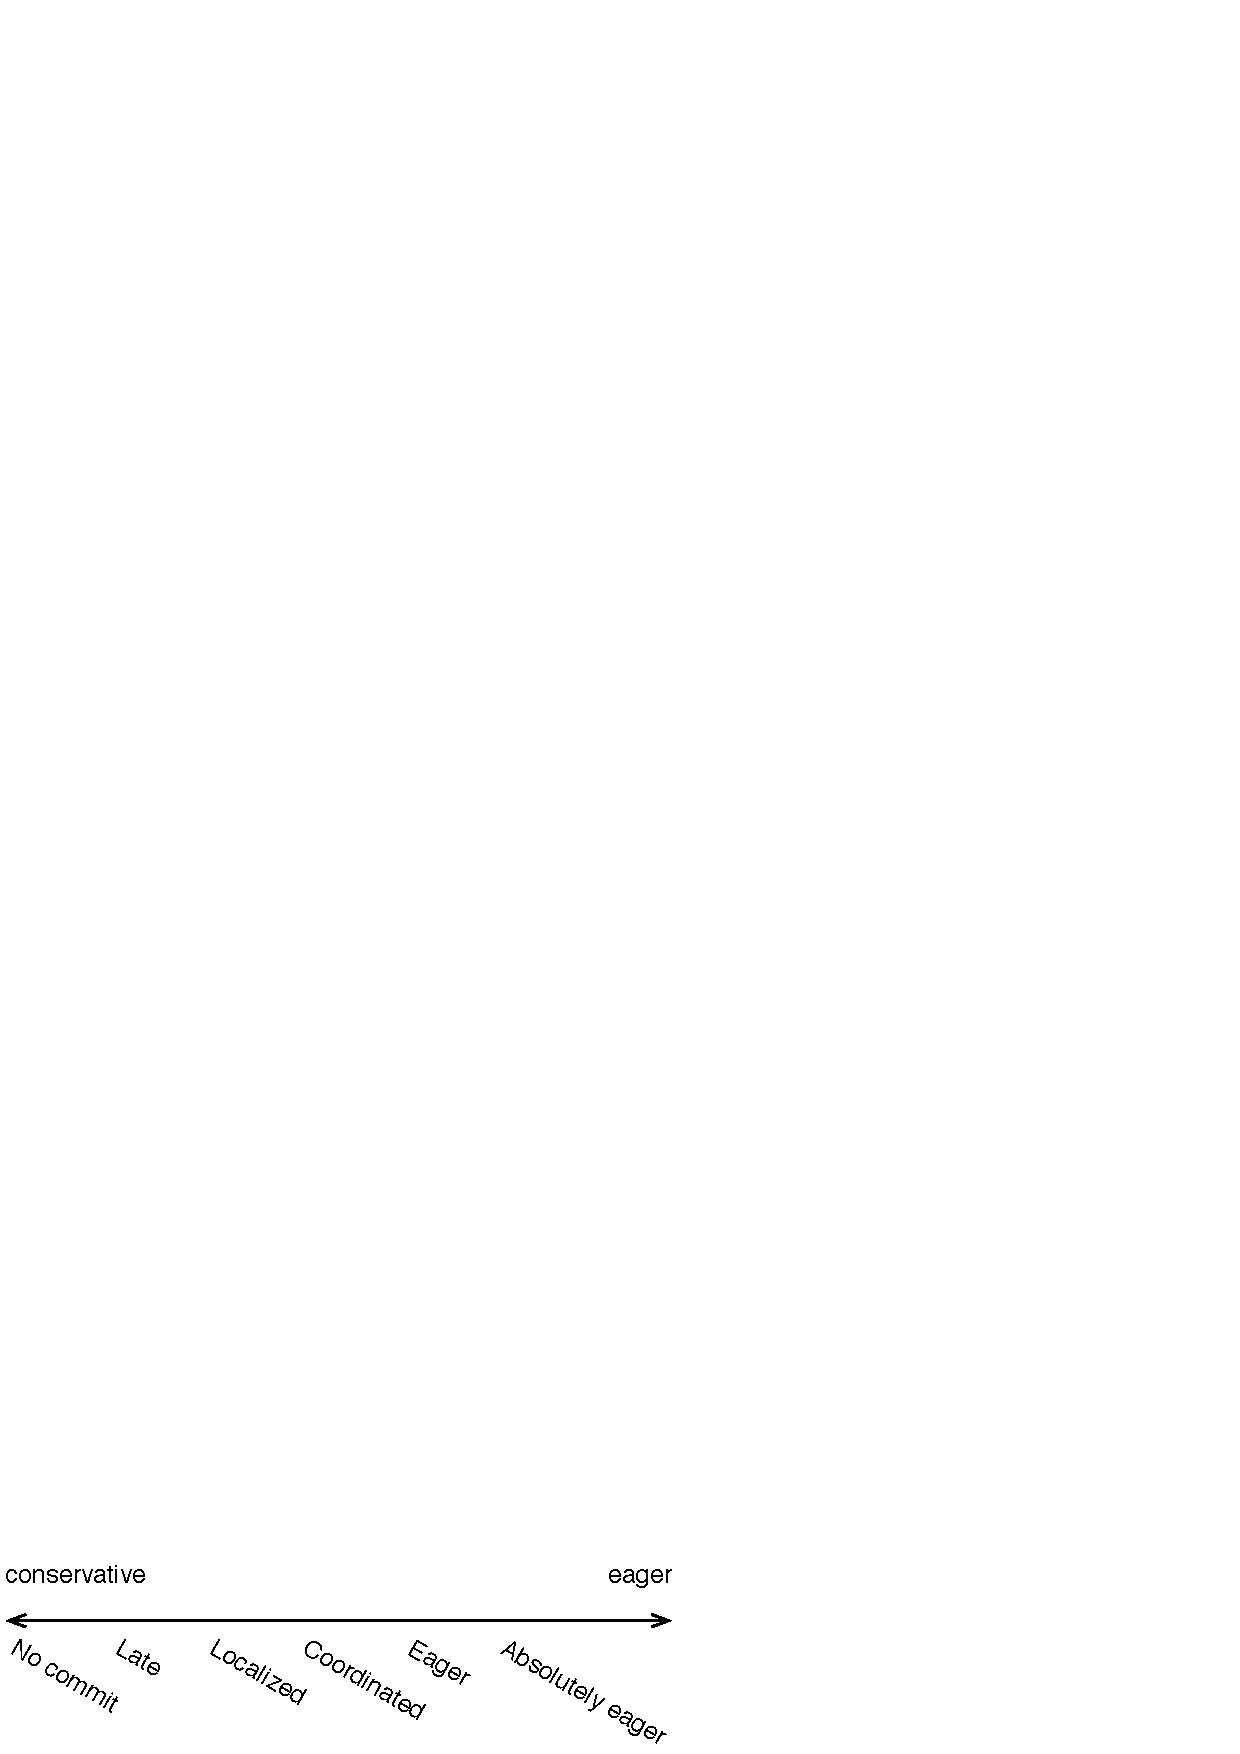
\includegraphics[width=0.4\textwidth]{commit-spectrum}
  \caption{Approximate Spectrum of Commit Semantics}
  \label{fig:commit-spectrum}
\end{figure}

Commits are used to control the run-time behavior,
mostly to prune choices for the purpose of performance.
The commit semantics described in Section \ref{sec:rules} and
in \figref{fig:rules} is called {\em localized commit} as it restricts
the scope of pruning to be of height 1 only.  $\cm$ by agent $X$ cannot
prune until the direct parent of the committed world is $\oplus_X$.
$\cu$ kills the current world immediately without coordination with other worlds.

Besides localized commit, in this section, we identify a number of other possible commit
semantics. They differ in their eagerness to prune the worlds.
They are ordered roughly from the most eager to the most conservative:
{\em absolutely eager commit}, {\em eager commit}, {\em coordinated commit}, {\em late commit}
and {\em no commit} (See \figref{fig:commit-spectrum}).
%The semantics of commits may be different and there are also 4 other commit semantics in order to support different types of pruning.
%They are the absolutely eager commit, the eager commit, the late commit, and the coordinated commit.
%Different commit semantics vary between the range of being conservative and eager, which is depicted in Figure \ref{fig:commit-spectrum}, where the ``none'' means no commit at all (i.e. to generate all the combinatorial choices).
%
We compare and contrast the behavior of these commit semantics
using the dining philosopher example and reason why localized commit
is the chosen semantics in the calculus.
Here we are only concerned with the shape of the tree structures
after different commits and ignore the details in the world (leaf nodes).
The initial structure is in \figref{fig:cmcmp:init},
and let's see the effect of $B$ committing in $w_1$.
\begin{description}
  \item[Absolutely eager commit] is the most aggressive form of commit and
as soon as one agent commits in one of the worlds,
it kills {\em all} the other worlds. As illustrated in
\figref{fig:cmcmp:abs}, system immediately prunes the whole sub-tree.

  \item[Eager commit] is less aggressive and kills the branch on the right
immediately once there is a commit in the branch on the left.
\footnote{Note that the terms ``left branch'' and ``right branch'' in this
discussion are symbolic and can be used interchangeably.}
This can be seen in \figref{fig:cmcmp:eager}.

  \item[Late commit] kills the branch on the right only if all occurrences
(not necessarily in the same scope) of the (syntactically) left branch commit.
In the example, it requires $B$ commits not only in $w_1$,
but also in $w_2$, $w_5$ and $w_7$ and prunes all the right-hand side of
$\oplus_B$ (\figref{fig:cmcmp:late}).

  \item[Coordinated commit] proposed in our previous work \cite{JaffarYZ07}
is a compromise between the eager commit and the late commit, which does not
kill the alternative choice until $\cm$ of this choice has been reached in
\emph{all} worlds in the {\em scope} of the choice construct.
In our example, this requires $B$ commits in both $w_1$ and $w_2$ and prunes
in the same way as the eager commit (\figref{fig:cmcmp:coord}).
%(i.e. the conjunctive view $\mathcal{CV}$); $\cu$ also uses $\mathcal{CV}$

  \item[No commit] is the naive behavior of ignoring all the $\cm$ or $\cu$
in the program. The net effect of this is that the universe can only grow and
doesn't shrink by itself even if all agents have reached completion and exit in all worlds.
The advantage of this is that if there is a solution for all the agents, this semantics
will find it, the disadvantage is the computation space is exponential.
If no-commit semantics is used, in this example, the shape of the tree
remains the same as the initial structure till the end.
To reclaim system resources, system could employ a global collapse rule below
to reduce a galaxy that has no more agents to a single world. And due to the
exit semantics and Property \ref{prop-exit},
any world in this galaxy can become the new galaxy.
\[
    \tag{\sc Collapse}\label{rule:collapse}
    \frac
    {\langle [], d, s \rangle \in leaves(G) }
    {G \gto \langle [], d, s \rangle}
\]


\item[Localized commit] cannot prune until $C$ commits in $w_1$ as well, because the reason for $B$ to commit in $w_1$ may be that $C$ lives in $w_1$. When $C$ commits in $w_1$, the tree structure becomes an intermediate state as shown in the left-hand side of Figure \ref{fig:cmcmp:local}. Then the pending commit from $B$ is executed and prunes in the same way as the absolutely eager commit eventually (right-hand side of Figure \ref{fig:cmcmp:local}). It is more conservative but can kill as many as the absolutely eager commit.
\end{description}

\begin{figure*}
\centering\small
\subfigure[Initial galaxy structure]{\label{fig:cmcmp:init}
\begin{minipage}{0.325\textwidth}
\Tree[.$\oplus_A$
    [.$\oplus_{B_1}$
        [.$\oplus_{C_1}$
            $w_1$
            $w_2$
        ]
        [.$\oplus_{C_2}$
            $w_3$
            $w_4$
        ]
    ]
    [.$\oplus_{C_3}$
        [.$\oplus_{B_2}$
            $w_5$
            $w_6$
        ]
        [.$\oplus_{B_3}$
            $w_7$
            $w_8$
        ]
    ]
]
\end{minipage}
}
\subfigure[Absolutely eager commit]{\label{fig:cmcmp:abs}
\begin{minipage}{0.195\textwidth}
\Tree[.$\oplus_A$
    $w_1$
    [.$\oplus_{C_3}$
        [.$\oplus_{B_2}$
            $w_5$
            $w_6$
        ]
        [.$\oplus_{B_3}$
            $w_7$
            $w_8$
        ]
    ]
]
\end{minipage}
}
\subfigure[Eager commit]{\label{fig:cmcmp:eager}
\begin{minipage}{0.225\textwidth}
\Tree[.$\oplus_A$
    [.$\oplus_{C_1}$
        $w_1$
        $w_2$
    ]
    [.$\oplus_{C_3}$
        [.$\oplus_{B_2}$
            $w_5$
            $w_6$
        ]
        [.$\oplus_{B_3}$
            $w_7$
            $w_8$
        ]
    ]
]
\end{minipage}
}
\subfigure[Late commit]{\label{fig:cmcmp:late}
\begin{minipage}{0.21\textwidth}
\centering
\begin{tabular}{c}
\\
\Tree[.$\oplus_A$
    [.$\oplus_{C_1}$
        $w_1$
        $w_2$
    ]
    [.$\oplus_{C_3}$
        $w_5$
        $w_7$
    ]
] \\ \\ \\
\end{tabular}
\end{minipage}
}
\subfigure[Coordinated commit]{\label{fig:cmcmp:coord}
\begin{minipage}{0.25\textwidth}
\Tree[.$\oplus_A$
    [.$\oplus_{C_1}$
        $w_1$
        $w_2$
    ]
    [.$\oplus_{C_3}$
        [.$\oplus_{B_2}$
            $w_5$
            $w_6$
        ]
        [.$\oplus_{B_3}$
            $w_7$
            $w_8$
        ]
    ]
]
\end{minipage}
}
\subfigure[Localized commit]{\label{fig:cmcmp:local}
\begin{tabular}{cccc}
$\quad$
&
\begin{minipage}{0.27\textwidth}
\Tree[.$\oplus_A$
    [.$\oplus_{B_1}$
        $w_1$
        [.$\oplus_{C_2}$
            $w_3$
            $w_4$
        ]
    ]
    [.$\oplus_{C_3}$
        [.$\oplus_{B_2}$
            $w_5$
            $w_6$
        ]
        [.$\oplus_{B_3}$
            $w_7$
            $w_8$
        ]
    ]
]
\end{minipage}
&
$\Rightarrow$
&
\begin{minipage}{0.18\textwidth}
\Tree[.$\oplus_A$
    $w_1$
    [.$\oplus_{C_3}$
        [.$\oplus_{B_2}$
            $w_5$
            $w_6$
        ]
        [.$\oplus_{B_3}$
            $w_7$
            $w_8$
        ]
    ]
]
\end{minipage}
\end{tabular}
}
\caption{Illustration of Different Commit Semantics}
\label{fig:cmcmp}
\end{figure*}

In general, the coordinated commit proposed previously \cite{JaffarYZ07}
has two disadvantages:
\begin{enumerate}
  \item The most attractive feature of coordinated commit is the ability to
  prune not only leaf worlds but also subtrees of worlds,
  but the condition for this to happen requires $\cm$ of this choice to be reached
  in the scope of the choice construct, in all worlds.
  However, it is costly to do so as it needs to maintain information
	of the {\em conjunctive views} of many data stores. \footnote{Conjunctive view
of a set of stores $D$ is the common data in $D$.}
  \item As shown in the following example, it may prune the only world
	where all agents can be satisfied.
\end{enumerate}

\begin{figure}[th]
  \centering
  \small\Tree[.$\oplus_X$
          [.$\oplus_Y$
            {$X:+\alpha.\cm_1$\\$Y:\underline{-\beta}.\cm$\\ \\ $(X_l Y_l)$}
            {$X:+\alpha.\cm_2$\\$Y:\underline{-\gamma}.\cm$\\ \\ $(X_l Y_r)$}
          ]
          [.$\oplus_Y$
            {$X:+\beta.\cm_3$\\$Y:-\beta.\cm_5$\\ \\$(X_r Y_l)$}
            {$X:+\beta.\cm_4$\\$Y:\underline{-\gamma}.\cm$\\ \\ $(X_r Y_r)$}
          ]
        ]
  \caption{Runtime Galaxy Structure for Programs $X$ and $Y$}
  \label{fig:commit-example}
\end{figure}


Let's consider the following simple program to understand why the localized commit is better
than the other pruning-based commit semantics and chosen as the default semantics in
our calculus. Suppose there are two agent programs $X$ and $Y$:
\begin{eqnarray*}
  X: & +\alpha.\cm\oplus +\beta.\cm \\
  Y: & -\beta.\cm\oplus -\gamma.\cm
\end{eqnarray*}

A possible runtime galaxy structure is shown in Figure \ref{fig:commit-example}
where $\oplus_X$ starts before $\oplus_Y$.
$X$ and $Y$ are subscripted with $l$ and $r$ which means
the left-hand side and the right-hand side respectively.
The underlined parts are blocked while all other operations can be executed successfully.
Subscripts of $\cm$ indicate the execution order of the commit actions.
Consider the effects of different commit semantics in Figure \ref{fig:commit-example}.

Absolutely eager commit prunes all the three worlds $X_l Y_r$, $X_r Y_l$ and $X_r Y_r$
when $\cm_1$ is executed.
Eager commit prunes both $X_r Y_l$ and $X_r Y_r$ when $\cm_1$ is executed.
Late commit waits until both $\cm_1$ and $\cm_2$ are executed and then prunes both
$X_r Y_l$ and $X_r Y_r$.
Coordinated commit is the same as late commit in this example.
Localized commit prevents $\cm_1$ and $\cm_2$ from pruning worlds
because the commits are issued by $X$ while the parent of $X_l Y_l$ and $X_l Y_r$ is $Y$;
only until $\cm_5$ is executed in world $X_r Y_l$ and
prunes $X_r Y_r$, the pending commit $\cm_3$ prunes both
$X_l Y_l$ and $X_l Y_r$.

\section{Analysis}
\label{sec:analysis}

% Analyze the main algo: time complexity, space complexity.
% Some properties to consider:
%
% \begin{itemize}
% \item give a bound on the total number of items suppressed;
% \item give a bound on the deviation in distribution from the original data;
% \item give a bound on the number of association rules that we eliminate;
% \item and what else??
% \end{itemize}

In this section, we show several interesting properties of our algorithm.
%in order to provide an all-aspect analysis of the problem and our algorithm.

%\begin{theorem}
%  The Optimal Suppression Problem in Definition \ref{def:osp} is NP-hard.
%\end{theorem}
%% TODO prove the whole problem hierarchy
%\begin{proof}
%  TODO
%\end{proof}

\begin{lemma}
\label{lemma:rule}
  If the inference $\mathcal{A}(q,a)$ is safe,
  then  $\mathcal{A}(q,a, b_1,b_2,\dots,b_n)$ is safe for any sequence of $\{b_i\}$.
\end{lemma}
\begin{proof}
  \begin{align*}
    \text{$q\rightarrow a$ is safe}
    \Rightarrow
    &\, \frac{\csize(q\cup\{a\})}{\csize(q)} \le \rho \\
    \Rightarrow
    &\, \csize(q\cup\{a\}) \le \rho\cdot\csize(q)
  \end{align*}
  \begin{align*}
    &\, (q\cup\{a\}) \subset (q\cup\{a, b_1,b_2,\dots,b_n\}) \\
    \Rightarrow
    &\,  \csize(q\cup\{a, b_1,b_2,\dots,b_n\}) \leq \csize(q\cup\{a\}) \le \rho\cdot\csize(q) \\
    \Rightarrow
    &\, \frac{\csize(q\cup\{a, b_1,b_2,\dots,b_n\}}{\csize(q)} \le \rho \\
    \Rightarrow
    &\, \text{$q\rightarrow a, b_1,b_2,\dots,b_n$ is safe}
  \end{align*}
\end{proof}

Lemma \ref{lemma:rule} shows that we do not have to consider rules with consequent of length 2 or longer.

\begin{lemma}%[Correctness of partitioning]
\label{CorrectnessOfPartitioning}
  If $q$ is safe in both $T_1$ and $T_2$, then $q$ is safe in $T = T_1 \cup T_2$.
\end{lemma}
\begin{proof}
For any item $a$,
  \begin{align*}
   q~\text{is safe in}~T_1 &\Rightarrow \csize_{T_1}(q\cup\{a\}) \le \rho\cdot\csize_{T_1}(q) \\
   q~\text{is safe in}~T_2 &\Rightarrow \csize_{T_2}(q\cup\{a\}) \le \rho\cdot\csize_{T_2}(q)
  \end{align*}
  So \begin{align*}
   \csize_{T_1}(q\cup\{a\}) + \csize_{T_2}(q\cup\{a\}) &\le \rho\cdot\csize_{T_1}(q) + \rho\cdot\csize_{T_2}(q)
  \end{align*}
  And \begin{align*}
    \csize_T(q\cup\{a\}) &= \csize_{T_1}(q\cup\{a\}) + \csize_{T_2}(q\cup\{a\}) \\
    \csize_T(q) &= \csize_{T_1}(q) + \csize_{T_2}(q)
  \end{align*}
  So $$ \frac{\csize_T(q\cup\{a\})}{\csize_T(q)} \le \rho~\Rightarrow q~\text{is safe in}~T .$$
\end{proof}

\begin{theorem}
\label{CorrectnessOfPartialSuppressor}
  \PartialSuppressor always terminates with a correct solution.
\end{theorem}
\begin{proof}
We first prove that if the algorithm terminates, the suppressed table is safe.
Note that the algorithm can only terminates on Line \ref{line:partial-suppressor-break}
  in Algorithm \ref{algo:partialsuppressor}.
So the value of $u$ on Line \ref{line:partial-suppressor-if-u} must always be \FALSE
  until the record cursor $i$ exceeds the table size $|T|$.
That means both \HandleShortRecords and \HandleLongRecord always return
  a pair with \FALSE as the first element during some pass of scanning of the whole table.
For \HandleShortRecords, returning \FALSE on Line \ref{line:handle-short-return-false}
  in Algorithm \ref{algo:handleshort} indicates there is no unsafe \qid in the buffer $B$.
For \HandleLongRecord, returning \FALSE on Line \ref{line:handle-long-return}
  in Algorithm \ref{algo:handlelong} indicates all the \qids generated by \Enum are safe.
So these return values of the two functions indicate there is no unsafe \qid in the table.
Hence, the suppressed table is safe.

Then we prove that \PartialSuppressor always terminates by measuring the
  number of items left (denoted $l$) in the table after each step of suppression.
Initially, $l=l_0=\sum_{i=1}^{|T|} |T[i]|\le |D| |T|$.
We state that for every invocation of \SanitizeBuffer, Line \ref{line:sanitize-suppress}
  in Algorithm \ref{algo:sanitize} is always executed at least once.
So the value $l$ strictly decreases when \SanitizeBuffer is invoked.
And before the table becomes safe, \SanitizeBuffer will be invoked for
  every iteration of the loop in Algorithm \ref{algo:partialsuppressor}.
So $l$ strictly decreases for each loop iteration in \PartialSuppressor.
Because $l$ starts from a finite number which is at most $l_0=\sum_{i=1}^{|T|} |T[i]|$,
  \PartialSuppressor must terminate.
Otherwise there will be an infinite descending chain of all the $l$ values.

Now we prove that Line \ref{line:sanitize-suppress} in Algorithm \ref{algo:sanitize}
  is always executed once \SanitizeBuffer is invoked.
Whenever \SanitizeBuffer is invoked, it is guaranteed that there exists
  an unsafe \qid $q\in B$ (see Line \ref{line:handle-short-if-contains-unsafe} in Algorithm \ref{algo:handleshort}
  and Line \ref{line:handle-long-if-contains-unsafe} in Algorithm \ref{algo:handlelong}).
$q$ is unsafe so that there always exists an item $e\in\linked(q)$ such that $P(e|q)>\rho$,
  i.e. \[ \frac{\csize(q\cup\{e\})}{\csize(q)}>\rho \Rightarrow \csize(q\cup\{e\})-\rho\cdot\csize(q)>0 .\]
For $k$ on Line \ref{line:sanitize-k1} in Algorithm \ref{algo:sanitize},
  \[ k = |X|-\lfloor\rho\cdot\csize(q)\rfloor = \csize(q\cup\{e\})-\lfloor\rho\cdot\csize(q)\rfloor \ge 1 .\]
For $k$ on Line \ref{line:sanitize-k2} in Algorithm \ref{algo:sanitize},
  it is guaranteed that the number of deletions is at least 1
  because the rule $q\rightarrow e$ is unsafe and there must be some deletions to make it safe.
So $k\ge 1$ on Line \ref{line:sanitize-while-k} for the first time.
Thus the condition is satisfied and Line \ref{line:sanitize-suppress} is executed.
\end{proof}

\begin{corollary}
The divide-and-conquer optimization \SplitData is correct.
\end{corollary}
\begin{proof}
It follows directly from Lemma \ref{CorrectnessOfPartitioning} and
Theorem \ref{CorrectnessOfPartialSuppressor}.
\end{proof}

%\begin{theorem}
%Let %$M = |T|$ be the size of table $T$,
%$l$ be the average record length,
%$c = r_r r_d$ where $r_r$ is the regression rate and $r_d$ is the qid duplicate rate.
%The average time complexity of \PartialSuppressor is
%\[ O(c \cdot 2^l |T|^2 l (\bmax (1-\rho) + l)). \]
%\end{theorem}
%\begin{proof}
%{\small\begin{verbatim}
%  general idea:
%  l1 <- estimate the number of iterations
%    for the loop in algorithm 1 -- assume
%    there is a parameter: regression ratio
%  may have to assume the data in some distribution
%    (e.g. power-law) -- related to Figure 1
%    count the number of invocations of HandleShort
%      --> b_max
%    count the number of invocations of HandleLong
%  l2 <- estimate the number of iterations
%    for the loop in algorithm 3
%  l1+l2 -> the number of invocation of SanitizeBuffer
%  estimate complexity of SanitizeBuffer
%  estimate complexity of line 7 to 13 in algorithm 3
%    (related to distribution in Figure 2)
%  estimate the complexity of UpdateBuffer
%\end{verbatim}}]

%Let $n_1$ be the number of short records,
%$n_2$ be the number of long records,
%$p(i)$ be the probability of a record being length $i$,
%$l_m$ be the maximum record length,
%$t=1-\rho$.
%
%Let $v_1$ be the number of invocations of \HandleShortRecords.
%In the process of generating qids and filling them into the qid buffer $B$,
%duplicates cannot be counted.
%If duplicates are allowed, the number of qids generated by a record is
%just $r=\sum_{i=1}^{\lmin-1} p(i)\cdot\#qid(i)$ where
%$\#qid(i)$ is the expected number of qids generated by a record of length $i$.
%Then $\bmax/r$ records are used to fill the buffer (duplicates allowed).
%So roughly $v_1=\frac{n_1\cdot r}{\bmax r_d}$ times to consider all distinct qids
%in short records, for a single pass.
%
%For \HandleLongRecord, the number of invocations is $v_2=n_2$ if
%we do not take multiple passes of table scanning (i.e., the loop in algorithm 1) into consideration.
%Assume the loop in \HandleLongRecord is iterated for $v_3$ times, then \SanitizeBuffer is
%roughly invoked for $v_1 + v_2 v_3$ times.
%
%There are 4 major parts in the computation. We will consider them one by one.
%
%The first part is Line 4 to 7 in Algorithm 2, since the buffer capacity is $\bmax$,
%the maximum number of iterations here is roughly $\bmax r_d$.
%\HandleShortRecords will be invoked for $v_1$ times, so
%the total time cost by this part of computation is roughly $v_1 \bmax r_d$.
%
%The second part is \UpdateBuffer in Algorithm 2. For the invocation
%$\UpdateBuffer(B, T, i, j, K, L)$, the purpose is to update $K$ and $L$
%by considering qids in records $T[i..j]$ which are also in $B$.
%So a single call invocation of \UpdateBuffer costs roughly $(j-i+1)|B|$.
%Hence, the total time cost by this part of computation is roughly
%$v_1 (|T| - \frac{\bmax}{r}) \bmax$.
%
%The third part is Line 7 to 13 in Algorithm 3. Note that in reality
%the computation from Line 10 to 12 can be done at the same time when
%calculating Line 8. And in the worst case, the total time cost by calculating
%these intersections is $\dnum l_m |T|$. And the total time cost by
%this part of computation is $v_2 v_3 \dnum l_m |T|$.

%The fourth part is all the invocations of \SanitizeBuffer.
%For a single invocation of \SanitizeBuffer, there are two sub-parts to consider.
%The first sub-part is the intersection calculation on Line 5 in Algorithm 4,
%which costs roughly $l |T|$.
%The second sub-part is the computation from Line 14 to 25 in Algorithm 4,
%which costs roughly $k |B|$, where $k$ is determined on Line $9$.
%In the worst case, $k= t |T|$.
%So for a single invocation of \SanitizeBuffer, the time cost is roughly
%$|B| r_r l (|T| L + t |T| |B|)$ where $|B|$ is the size of the buffer.
%Because \SanitizeBuffer is invoked $v_1$ times in \HandleShortRecords,
%with buffer size $\bmax$, and $v_2 v_3$ times in \HandleLongRecord,
%with buffer size $\dnum$,
%the total time cost by this part of computation is roughly
%$v_1 \bmax r_r l (l |T| + t |T| \bmax) + v_2 v_3 \dnum r_r l (l |T| + t |T| \dnum)$.
%
%Summing up these four parts we can get the following time cost.
%\begin{align*}
%  n_1 r
%+ \frac{n_1 (r |T| - \bmax)}{r_d}
%+ \frac{n_1 |T| r l r_r (\bmax t + l)}{r_d} \\
%+ l_m |T| n_2 \dnum v_3
%+ l |T| n_2 \dnum v_3 r_r (l + \dnum t)
%\end{align*}
%By eliminating non-denominating terms, we get the order of \[ O(c \cdot 2^l |T|^2 l (\bmax (1-\rho) + l) ) .\]
%\end{proof}
%
%For a given dataset, the expected time complexity is actually quadratic to the size of the table.

%\begin{theorem}
%  The space complexity of \PartialSuppressor on table $T$ is \[ O(\sum_{i=1}^{|T|} |T[i]| + \bmax) .\]
%\end{theorem}
%\begin{proof}
%Let $N = \sum_{i=1}^{|T|} |T[i]|$, then $N$ is the sum of the numbers
%of all item occurrences.
%This term is easy to explain since the algorithm has to store
%the original table $T$.
%So we only need to consider local data structures
%created in \PartialSuppressor
%and related functions for the term $O(\bmax)$.
%
%For \PartialSuppressor, the most significant memory cost is from the \qid buffer of size $\bmax$.
%For \HandleShortRecords, there is only $O(1)$ extra memory space for loop variables like $j$.
%For \HandleLongRecord, there is also $O(1)$ extra memory cost.
%For \SanitizeBuffer, except for the $O(1)$ memory space for local variables, it also involves
%  the storage of $\linked(\cdot)$ and $\csize(\cdot)$.
%Because all the \qids updated are from the buffer $B$, the total number of \qids being active at any time
%  is no greater than the capacity of the buffer, i.e. $\bmax$.
%In order to keep the information of $\linked(\cdot)$ and $\csize(\cdot)$,
%  there will be $O(\bmax)$ extra memory space used.
%\end{proof}

%\begin{theorem}
%  The algorithm suppresses at most $O(xxx)$ item occurrences on average.
%\end{theorem}
%\begin{proof}
%  TODO
%\end{proof}
%
%\KZ{Say something about the property of regression?}
%
%\KZ{A property for DnC time performance? The experiment seems to show that
%time decreases exponetially with $t_{max}$ for Retail, which is amazing!}

%\begin{property}
%  Idea: distribution similarity ...
%\end{property}
%\begin{proof}
%  TODO
%\end{proof}

